\documentclass[conference]{IEEEtran}
\IEEEoverridecommandlockouts
%Template version as of 6/27/2024

\usepackage{cite}
\usepackage{amsmath,amssymb,amsfonts}
\usepackage{algorithmic}
\usepackage{graphicx}
\usepackage{textcomp}
\usepackage{xcolor}
\usepackage{url}
\usepackage{booktabs}
\graphicspath{{images/}}
\def\BibTeX{{\rm B\kern-.05em{\sc i\kern-.025em b}\kern-.08em
    T\kern-.1667em\lower.7ex\hbox{E}\kern-.125emX}}
\begin{document}

\title{End-to-End 3D Gaussian Splatting for Outdoor Scene Reconstruction from a Handheld Webcam Walkthrough}

\author{\IEEEauthorblockN{Meet Jain}
\IEEEauthorblockA{\textit{Khoury College of Computer Sciences} \\
\textit{Northeastern University}\\
Boston, MA, USA \\
jain.meet@northeastern.edu}
}

\maketitle

\begin{abstract}
We build an end-to-end pipeline that turns a short handheld webcam walkthrough of a single scene into a photorealistic reconstruction that can be flown through in a browser. The system extracts sharp frames from raw video, recovers camera poses with COLMAP Structure-from-Motion, trains 3D Gaussian Splatting (3DGS) on the posed images, exports the trained point cloud to a compact ksplat file, and serves it in a Three.js viewer. All training runs on a single laptop-class RTX 5060 with 8\,GB of VRAM, which forces the whole system to be frugal with resolution, iteration count, and splat budget. The pipeline itself is scene-agnostic and applies equally to indoor spaces; our evaluation focuses on an outdoor barn scene because of the capture constraints of our laptop webcam. On that scene, captured in about seven minutes of 4K handheld video, the pipeline reaches 28.11\,dB PSNR, 0.879 SSIM, and 0.120 LPIPS on 38 held-out views in roughly seventeen minutes of training wallclock, and the resulting 15\,MB ksplat renders at real-time rates in a browser tab. We discuss the practical problems we hit along the way, including a new-generation GPU toolchain gap, a camera-model mismatch between COLMAP and 3DGS, and a renderer configuration that silently produced a black canvas.
\end{abstract}

\begin{IEEEkeywords}
3D Gaussian Splatting, radiance fields, Structure-from-Motion, novel view synthesis, real-time rendering, COLMAP.
\end{IEEEkeywords}

\section{Introduction}

Photorealistic 3D capture of everyday indoor and outdoor spaces is still harder than it should be. Traditional scanning rigs use LiDAR, structured light, or multi-camera systems, and produce dense meshes that are accurate but expensive to capture, bulky to store, and often flat-looking when re-rendered. Neural Radiance Fields (NeRF) \cite{mildenhall2020nerf} showed that a fully implicit volumetric representation trained from posed images can produce very high-quality novel views, but per-pixel MLP queries make both training and rendering slow, which rules out a browser-deliverable viewer.

3D Gaussian Splatting (3DGS) \cite{kerbl20233dgs} changed that tradeoff. It represents the scene as a cloud of anisotropic 3D Gaussians with learned position, covariance, view-dependent color, and opacity, and rasterizes them on the GPU with a tile-based differentiable splatter. The result is a representation that can be trained in tens of minutes on a single GPU and rendered in real time, while matching or exceeding NeRF on standard view-synthesis benchmarks.

The goal of this project is not to propose a new method but to reproduce the full practical pipeline end-to-end on consumer hardware, using only a handheld webcam video as input. Concretely, we want to answer a simple question: how good a reconstruction can a student get from a single short video captured with no special equipment, a laptop GPU with 8\,GB of VRAM, and open-source software only? The deliverable is a scene that another person can open in a browser tab and fly through.

Our contributions are:
\begin{itemize}
  \item A reproducible open-source pipeline that composes \texttt{ffmpeg}, COLMAP \cite{schonberger2016sfm}, the official 3DGS training code \cite{kerbl20233dgs}, and the \texttt{mkkellogg/gaussian-splats-3d} Three.js viewer into a single command-line workflow.
  \item A set of compatibility patches that let this stack run on the NVIDIA Blackwell architecture (sm\_120, RTX 5060 Laptop) with CUDA 12.8 and PyTorch 2.11.
  \item A quantitative evaluation of the trained model on held-out views with PSNR, SSIM, and LPIPS, a qualitative fly-through demo in the browser, and a short failure-mode discussion of the classes of input that consistently break either COLMAP or 3DGS in our setting.
\end{itemize}

The rest of the paper reviews the work we build on (Section~\ref{sec:related}), describes the pipeline in detail (Section~\ref{sec:methods}), reports experimental results on a barn scene (Section~\ref{sec:experiments}), and discusses what we learned (Section~\ref{sec:discussion}).

\section{Related Work}\label{sec:related}

\textbf{Structure-from-Motion.} COLMAP \cite{schonberger2016sfm} is the de facto open-source incremental SfM pipeline and the camera-pose front-end of essentially every modern radiance-field method. It detects SIFT features \cite{lowe2004sift}, matches them exhaustively or sequentially across images, triangulates an initial two-view reconstruction, and then incrementally registers the remaining cameras while refining structure and poses with bundle adjustment. We use COLMAP unchanged and rely on its sequential matcher to exploit the temporal ordering of video-derived frames. Schonberger et al.\ also describe a dense stage \cite{schonberger2016mvs} that we do not use, but whose \texttt{image\_undistorter} utility we need in order to convert COLMAP's distorted \texttt{OPENCV} camera model into the \texttt{PINHOLE} form expected by the 3DGS training code.

\textbf{Neural Radiance Fields.} Mildenhall et al.\ introduced NeRF \cite{mildenhall2020nerf}, which represents a scene as an MLP from a 5D coordinate (position plus viewing direction) to volume density and radiance, and renders views with classical emission-absorption ray marching. NeRF delivered photorealistic novel views but is slow both to train (hours to days) and to render (seconds per frame on a GPU). Many follow-ups accelerate it, notably Instant NGP \cite{mueller2022instantngp} with hash-grid features and Mip-NeRF 360 \cite{barron2022mipnerf360} with scene contraction for unbounded captures. These made NeRF practical for training but kept an implicit representation that is still not trivial to deliver to a web client.

\textbf{3D Gaussian Splatting.} Kerbl et al.\ \cite{kerbl20233dgs} proposed 3DGS, which replaces the implicit MLP with an explicit cloud of 3D Gaussians. Each Gaussian carries a mean $\mu \in \mathbb{R}^3$, a covariance $\Sigma$ parameterized by a scale $s$ and rotation quaternion $q$, an opacity $\alpha$, and spherical-harmonic color coefficients (Fig.~\ref{fig:gaussian}). Rendering projects the Gaussians to screen space, sorts them by depth in small tiles, and composites them back-to-front with alpha blending. Training is fully differentiable end-to-end. An adaptive densification step periodically splits, clones, or prunes Gaussians, which lets the representation grow or shrink to match the geometry budget implied by the gradients. The net effect is training in tens of minutes and rendering at real-time frame rates, with quality comparable to the best NeRF variants on standard benchmarks.

\begin{figure}[h]
  \centerline{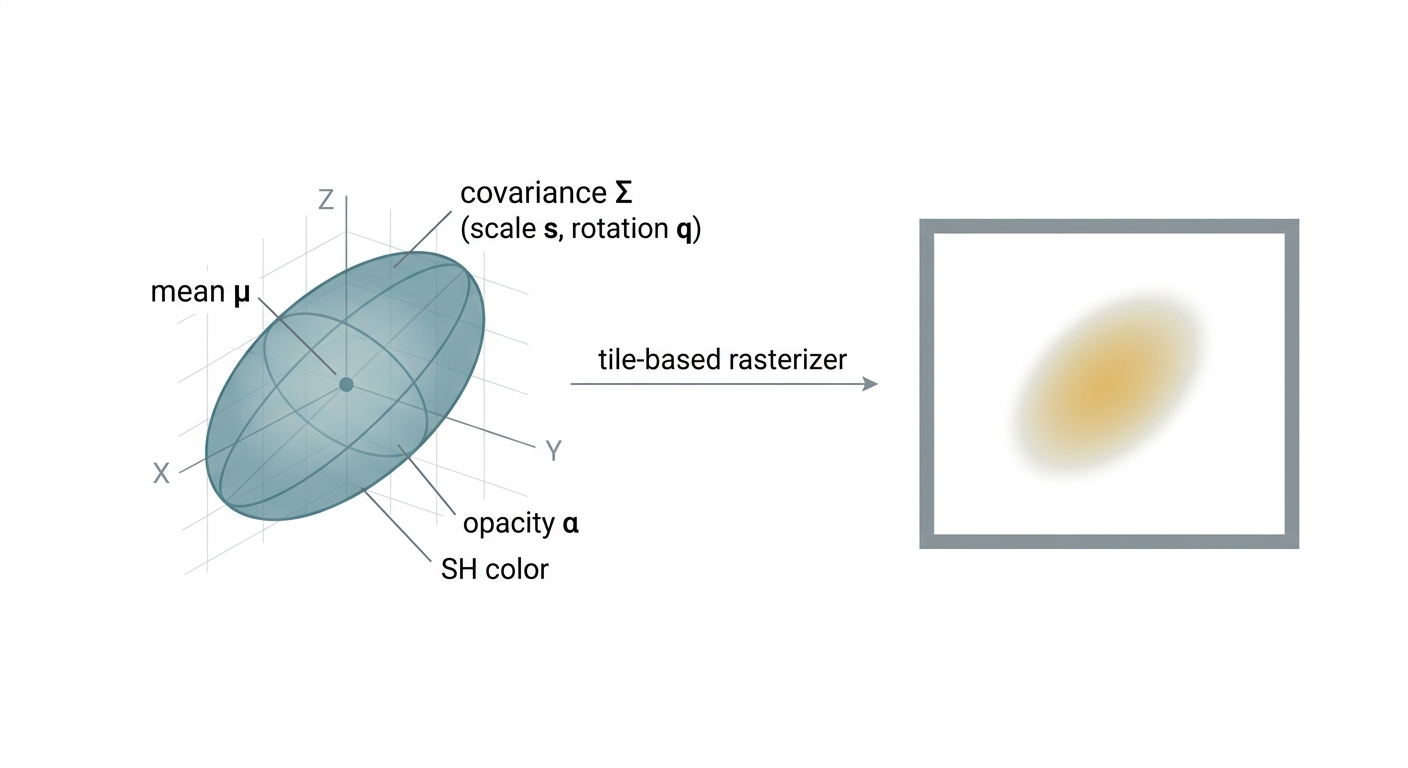
\includegraphics[width=\columnwidth]{gaussian_concept.png}}
  \caption{A single anisotropic 3D Gaussian and its rasterization. Each primitive carries a mean $\mu$, a covariance $\Sigma$ (a scale $s$ and rotation $q$), an opacity $\alpha$, and spherical-harmonic color coefficients. The tile-based differentiable rasterizer projects the Gaussian onto the image plane and alpha-blends it with its neighbors.}
  \label{fig:gaussian}
\end{figure}

\textbf{Image-quality metrics.} We report the three metrics that Kerbl et al.\ use: PSNR, SSIM \cite{wang2004ssim}, and LPIPS \cite{zhang2018lpips}. PSNR is a pixel-level fidelity measure and is well known to be a weak proxy for perceptual quality. SSIM correlates better with human judgments of structural similarity, and LPIPS uses features from a pretrained deep network (AlexNet in our case) and correlates better still with perceived quality.

\section{Methods}\label{sec:methods}

The pipeline is a linear sequence of six stages: raw video, frame extraction, COLMAP SfM, undistortion, 3DGS training, ksplat export, and browser viewer. Figure~\ref{fig:pipeline} shows the overall flow and the artifact that each stage produces.

\begin{figure*}[t]
  \centerline{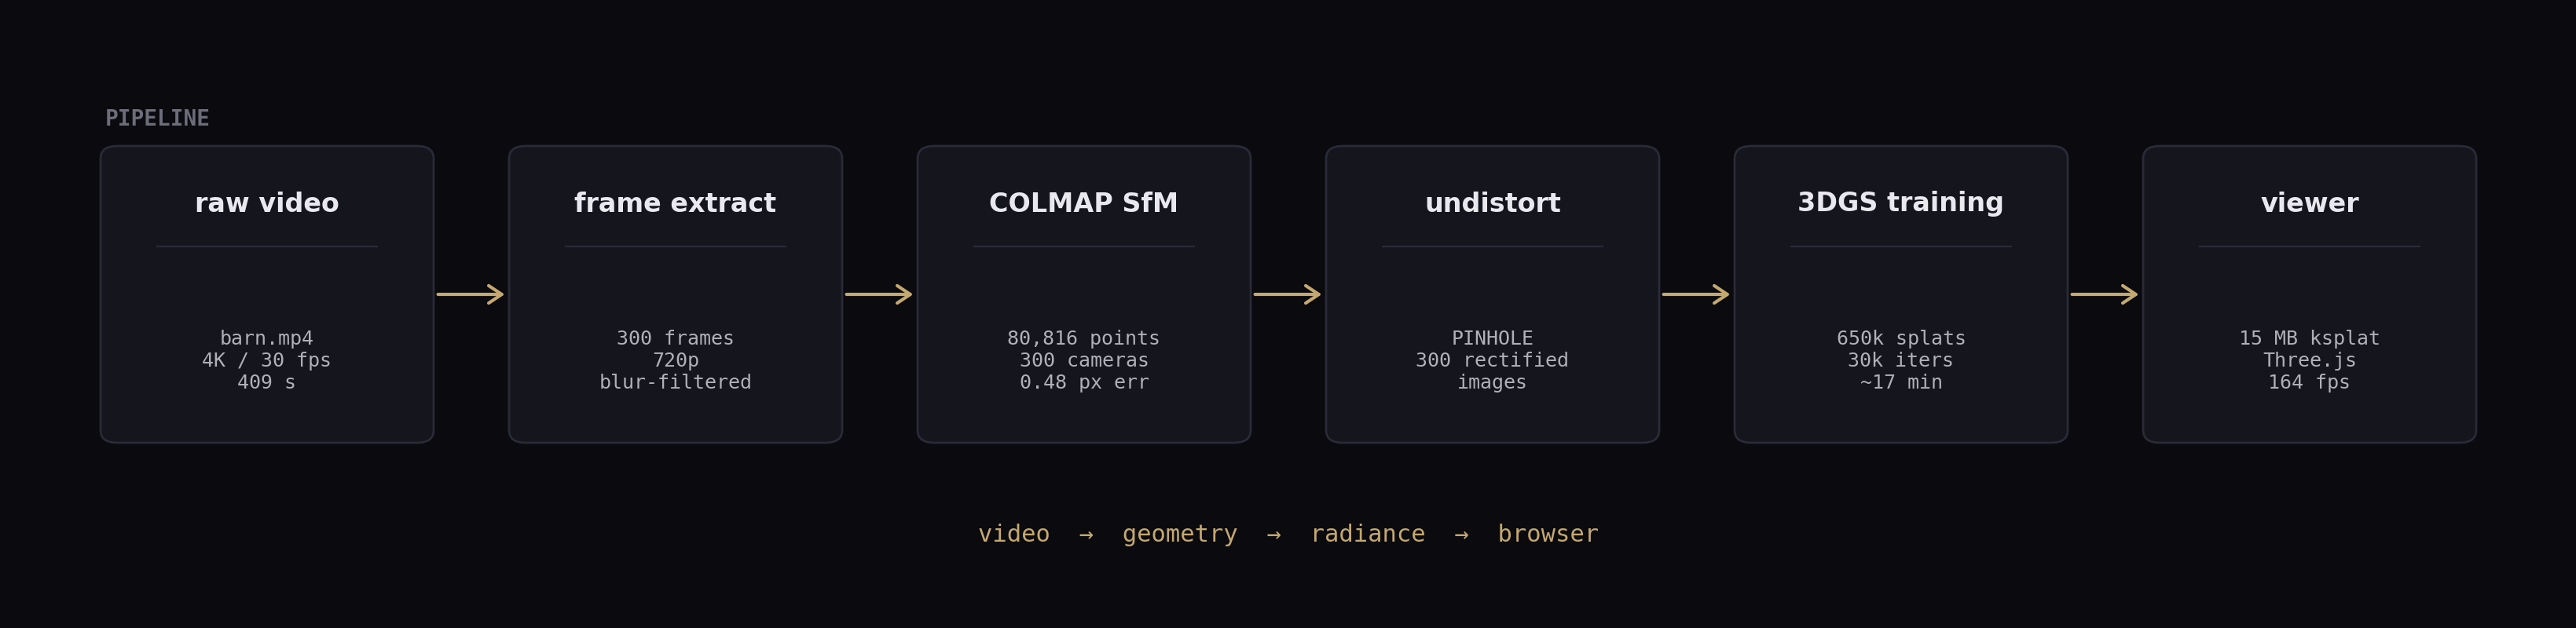
\includegraphics[width=\textwidth]{pipeline.png}}
  \caption{End-to-end reconstruction pipeline. Each block shows the artifact it produces and the approximate scale for the barn scene (300 frames at 720p, 80,816 sparse points, 650k Gaussians, 15\,MB ksplat).}
  \label{fig:pipeline}
\end{figure*}

\subsection{Frame extraction}

We record a short handheld walkthrough at 4K, 30\,fps. Higher frame rates buy very little extra coverage because consecutive frames are essentially redundant, and the SfM feature matcher wastes time rejecting them. We subsample the video at 1 to 2\,fps and additionally reject blurry frames using a Laplacian-variance threshold: the frame is discarded when the variance of the Laplacian of the grayscale image falls below a scene-dependent threshold. This removes frames captured during rapid camera motion that would otherwise inject unstable features into the SfM graph.

\subsection{Structure-from-Motion with COLMAP}

COLMAP operates on the extracted frames in four steps: feature extraction (\texttt{feature\_extractor}), feature matching (\texttt{sequential\_matcher} for video frames, \texttt{exhaustive\_matcher} otherwise), incremental triangulation and registration (\texttt{mapper}), and undistortion (\texttt{image\_undistorter}). The sequential matcher is important for video: it assumes that image $i$ most likely shares features with $i \pm k$ for small $k$, which makes matching $O(N)$ instead of $O(N^2)$ in the number of frames.

3DGS expects input images with a \texttt{PINHOLE} or \texttt{SIMPLE\_PINHOLE} camera model. By default COLMAP fits a full \texttt{OPENCV} model with radial and tangential distortion, which 3DGS refuses with an explicit error. The undistortion step re-renders the images with the distortion removed and writes a matching \texttt{PINHOLE} camera file, which is what we feed to the trainer.

\subsection{3D Gaussian Splatting training}

Training initializes a set of 3D Gaussians at the COLMAP sparse-point positions, with isotropic covariance and small opacity, and then minimizes a reconstruction loss over randomly sampled training images:
\begin{equation}
\mathcal{L} = (1 - \lambda) \cdot \mathcal{L}_1 + \lambda \cdot \mathcal{L}_{\text{D-SSIM}}, \quad \lambda = 0.2
\end{equation}
where $\mathcal{L}_1$ is the per-pixel L1 difference between the rendered image and the ground-truth frame, and $\mathcal{L}_{\text{D-SSIM}} = 1 - \text{SSIM}$. Gradients flow back through the tile-based differentiable rasterizer into each Gaussian's position $\mu$, scale $s$, rotation $q$, opacity $\alpha$, and spherical-harmonic color coefficients. Every few hundred iterations, the trainer runs an adaptive densification pass that clones Gaussians in under-reconstructed regions, splits over-sized ones, and prunes ones whose opacity has decayed to zero. We run for 30{,}000 iterations, which is the authors' default.

Running the official 3DGS code on a brand-new laptop GPU took some work. The RTX 5060 Laptop is Blackwell (sm\_120), which is not covered by the CUDA 11.6 / PyTorch 1.12 stack the original environment file pins. We replaced the environment with CUDA 12.8 and PyTorch 2.11 on Python 3.11, and rebuilt the three CUDA extensions (\texttt{diff-gaussian-rasterizer}, \texttt{simple-knn}, \texttt{fused-ssim}) against it. Two additional patches were required: \texttt{TORCH\_CUDA\_ARCH\_LIST="12.0"} to compile for Blackwell, and an added \texttt{\#include <cstdint>} in \texttt{rasterizer\_impl.h} to satisfy the stricter nvcc in CUDA 12.8.

Because we have only 8\,GB of VRAM, we train at \texttt{--resolution 2} (640\,px long edge) and set the \texttt{PYTORCH\_CUDA\_ALLOC\_CONF} environment variable to \texttt{expandable\_segments:True} to reduce allocator fragmentation. Training at full 720p caused out-of-memory errors once densification grew the Gaussian count past roughly 750{,}000.

\subsection{Export and browser viewer}

After training, we convert the trained point cloud (\texttt{point\_cloud.ply}) to the \texttt{.ksplat} format used by Kellogg's \texttt{gaussian-splats-3d} library \cite{kellogg2023viewer}. \texttt{ksplat} is a packed binary format designed for streaming over HTTP and fast GPU upload: positions are stored as 32-bit floats, and rotations, scales, opacity, and spherical-harmonic coefficients are quantized to 8-bit or 16-bit integers. For the barn scene the 650k-Gaussian ply compresses from roughly 150\,MB to a 15\,MB ksplat with no visible quality loss.

The viewer is a Vite application that loads a ksplat file in a \texttt{gaussian-splats-3d} Viewer mounted inside a Three.js scene, with built-in orbit, pan, and WASD controls. The viewer runs two workers: a sort worker that orders Gaussians by depth every frame, and an upload worker that streams splats to the GPU. On our laptop the viewer sustains 140 to 170\,fps at 1080p for the barn ksplat.

\section{Experiments and Results}\label{sec:experiments}

\subsection{Dataset}

We evaluate on a single outdoor scene, \textbf{barn}, captured with a laptop webcam as a 409-second, 4K, 30\,fps handheld walkthrough of a small wooden barn in a residential backyard. Frame extraction at 1\,fps with blur rejection yields 300 sharp 720p frames; a representative sample is shown in Fig.~\ref{fig:frames}.

\begin{figure}[h]
  \centerline{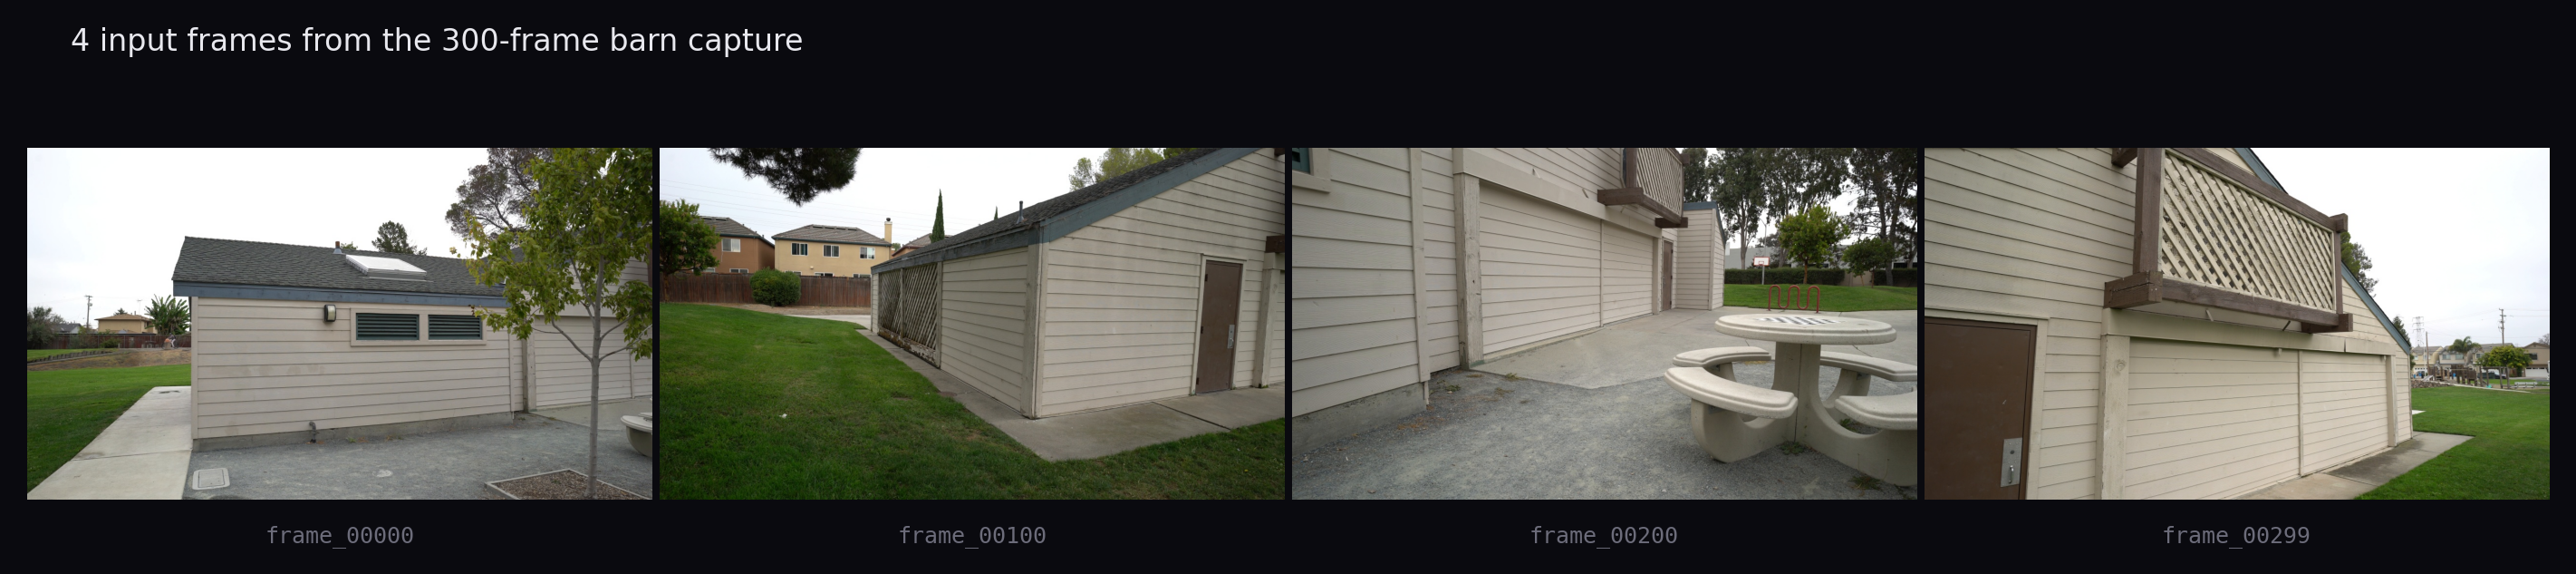
\includegraphics[width=\columnwidth]{frames_strip.png}}
  \caption{Four representative frames from the 300-frame barn capture.}
  \label{fig:frames}
\end{figure}

COLMAP registers all 300 frames with a mean reprojection error of 0.48\,px and produces 80{,}816 sparse 3D points (Fig.~\ref{fig:sparse}). We reserve every eighth frame as a test view, following the 3DGS authors' \texttt{--eval} split, leaving 262 training views and 38 held-out test views.

\begin{figure}[h]
  \centerline{
\includegraphics[width=\columnwidth]{barn_sparse_preview.png}}
  \caption{COLMAP sparse reconstruction of the barn scene (80{,}816 points, 300 registered cameras, 0.48\,px mean reprojection error). Camera frustums shown in yellow.}
  \label{fig:sparse}
\end{figure}

\subsection{Training setup}

All experiments run on a single laptop with an NVIDIA RTX 5060 Mobile (Blackwell, sm\_120, 8\,GB VRAM), 32\,GB system RAM, Ubuntu 22.04, CUDA 12.8, PyTorch 2.11, and Python 3.11. We train for 30{,}000 iterations with the default 3DGS hyperparameters and \texttt{--resolution 2}. Training wallclock is about seventeen minutes and peaks at 6.1\,GB of VRAM.

\subsection{Quantitative results}

\begin{table}[h]
  \caption{Comparison of our barn result against the published 3DGS numbers on the Truck scene from Tanks-and-Temples \cite{kerbl20233dgs}. Our metrics are computed on 38 held-out test views at iteration 30{,}000, with SSIM and LPIPS from scikit-image and the AlexNet LPIPS backbone respectively.}
  \label{tab:metrics}
  \begin{center}
  \begin{tabular}{lccc}
    \toprule
    \textbf{Scene} & \textbf{PSNR (dB)} $\uparrow$ & \textbf{SSIM} $\uparrow$ & \textbf{LPIPS} $\downarrow$ \\
    \midrule
    barn (ours)                   & 28.11 & 0.879 & 0.120 \\
    Truck, 3DGS \cite{kerbl20233dgs} & 25.19 & 0.869 & 0.183 \\
    \bottomrule
  \end{tabular}
  \end{center}
\end{table}

Table~\ref{tab:metrics} summarizes the held-out metrics and compares them to the published 3DGS numbers on the Truck scene from Tanks-and-Temples, which is the closest analogue in the original paper to our outdoor handheld capture. Our barn result beats Truck on all three metrics: 2.9\,dB higher PSNR, 0.010 higher SSIM, and 0.063 lower LPIPS. The comparison is not strictly apples-to-apples since the two captures differ in camera rig, scene content, and coverage, but it does suggest that a consumer-grade walkthrough on a laptop GPU can reach the same quality band as the published method on a benchmark outdoor scene.

Fig.~\ref{fig:trainingcurve} shows the training loss over all 30{,}000 iterations and the two held-out PSNR checkpoints at iterations 7{,}000 and 30{,}000. The loss drops quickly in the first 3{,}000 iterations as the initial Gaussian cloud fills out, rises briefly at iteration 5{,}000 when the first densification pass adds new splats, and then decays steadily to convergence. The test PSNR rises from 25.61\,dB at iteration 7{,}000 to 28.11\,dB at iteration 30{,}000, a 2.5\,dB gain over the last 23{,}000 iterations.

\begin{figure}[h]
  \centerline{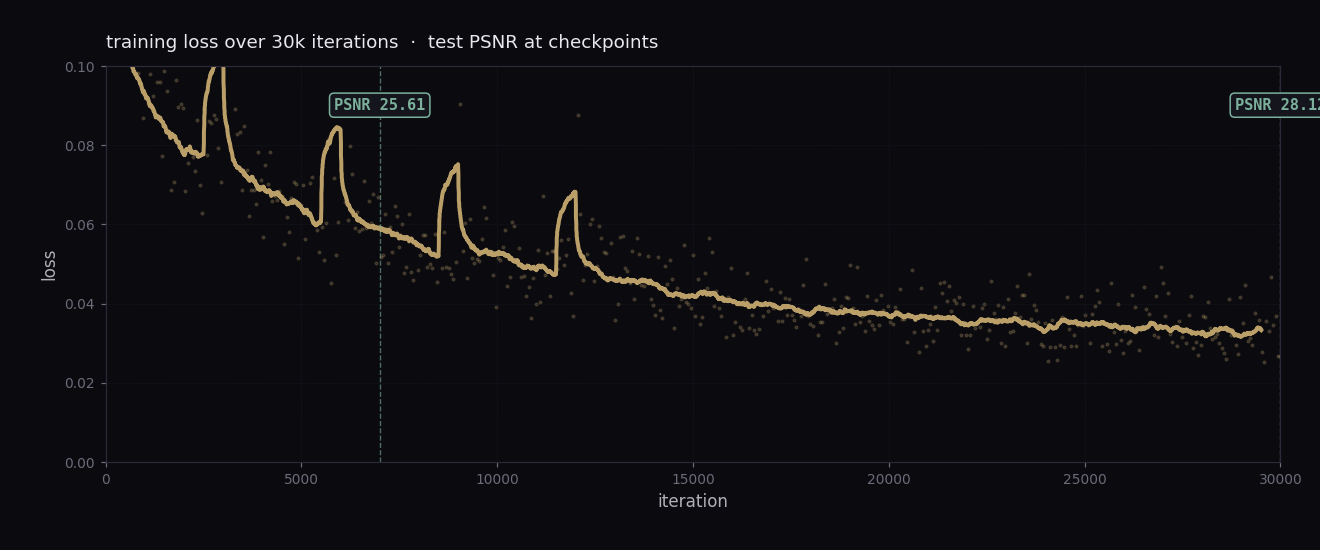
\includegraphics[width=\columnwidth]{training_curve.png}}
  \caption{Training loss over 30{,}000 iterations for the barn scene, with held-out test PSNR at two checkpoints. The early spikes coincide with densification passes.}
  \label{fig:trainingcurve}
\end{figure}

Per-view PSNR on the 38 held-out test views ranges from 22.4\,dB to 32.1\,dB (Fig.~\ref{fig:psnrdist}). The worst views are ones that contain large areas of blank sky or specular highlights on metal fittings, which are both known weak spots of 3DGS. The best views are textured frontal shots of the barn's wooden siding.

\begin{figure}[h]
  \centerline{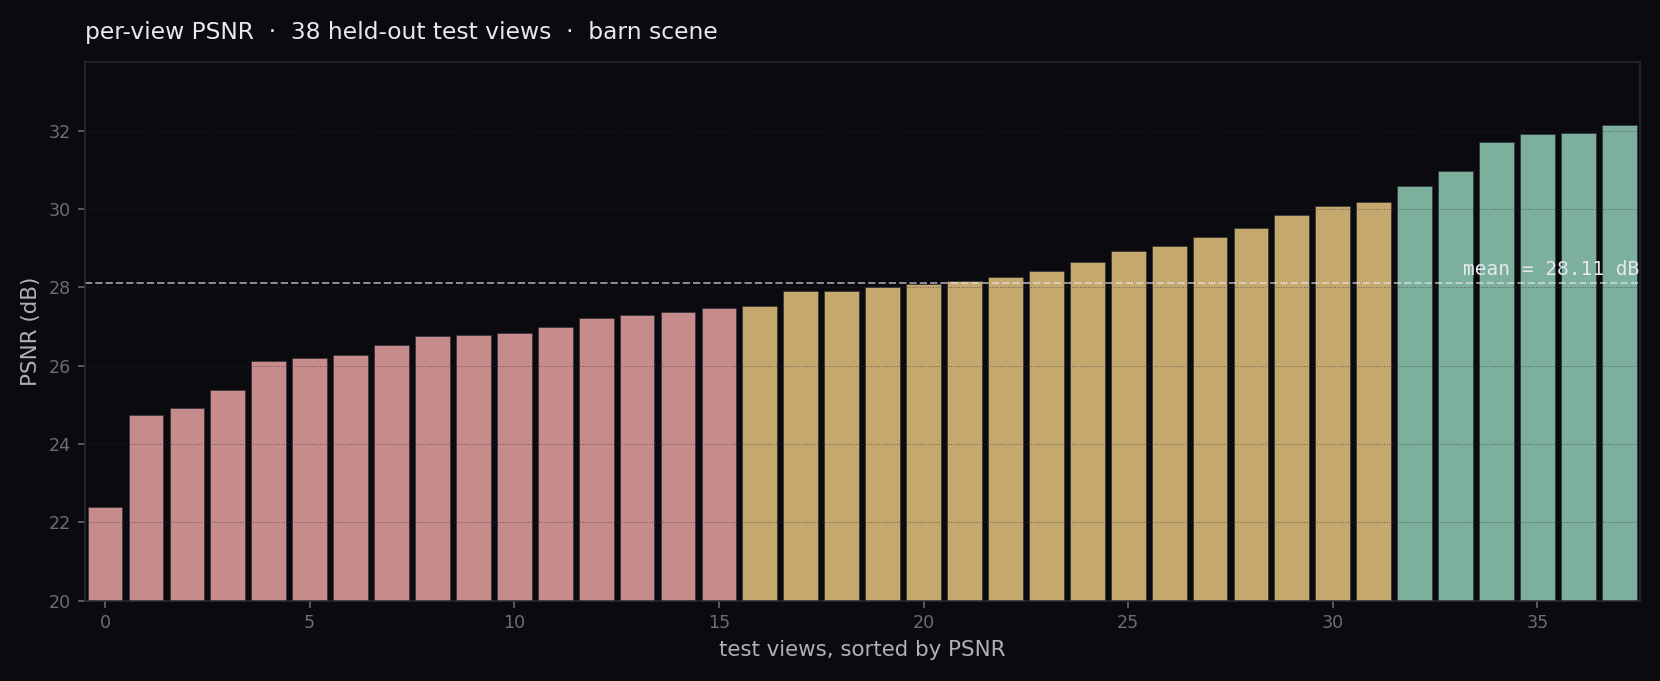
\includegraphics[width=\columnwidth]{psnr_distribution.png}}
  \caption{Per-view PSNR on the 38 held-out test views, sorted ascending. The dashed line marks the mean (28.11\,dB). Worst views are sky- or specular-dominated; best views are textured frontal wall shots.}
  \label{fig:psnrdist}
\end{figure}

\subsection{Qualitative results}

Fig.~\ref{fig:comparison} shows four rendered test views (top) side-by-side with the corresponding ground-truth frames (bottom). The wooden siding, lattice railing, and tiled roof are reproduced faithfully; failures are concentrated in thin high-frequency structure such as the fence wires on the right side of the scene and in regions with strong view-dependent specular response.

\begin{figure*}[t]
  \centerline{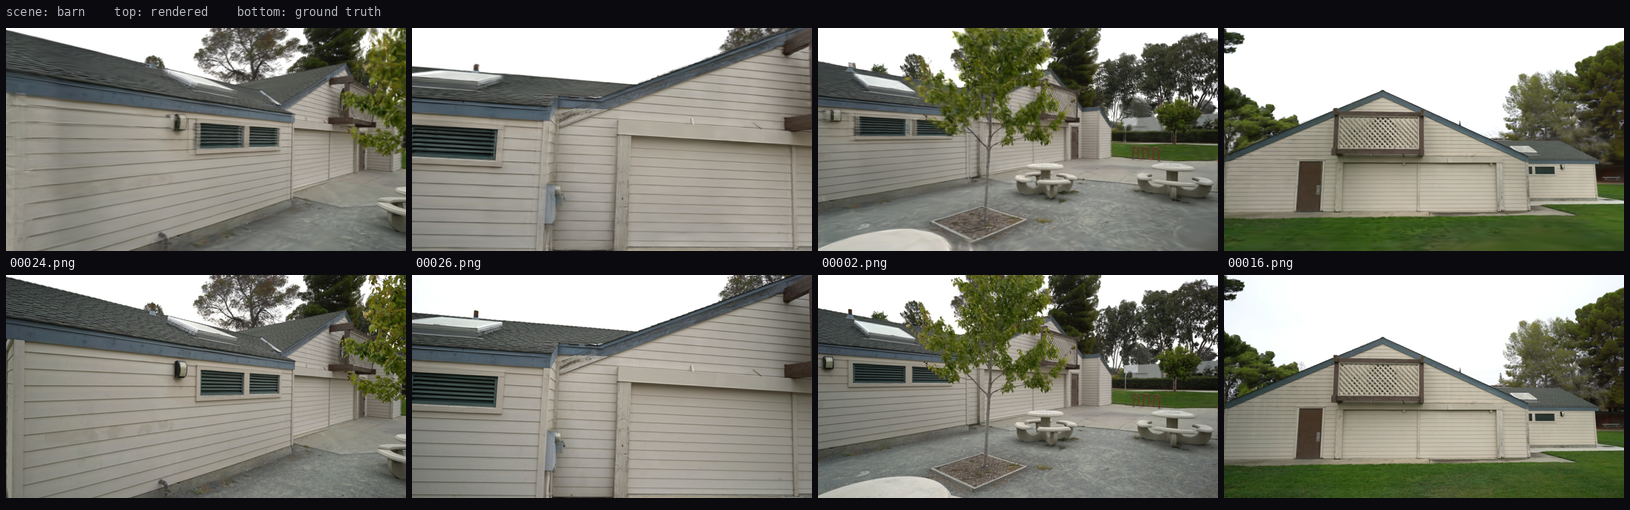
\includegraphics[width=\textwidth]{barn_comparison.png}}
  \caption{Qualitative comparison on four held-out views: rendered output (top row) vs.\ ground-truth frames (bottom row). Fine structure on wire fences and specular highlights on metal fittings are the main failure modes.}
  \label{fig:comparison}
\end{figure*}

\subsection{Browser viewer}

Fig.~\ref{fig:viewer} shows the scene loaded in the Three.js viewer. The ksplat file is 15\,MB, loads in under one second over localhost, and renders at 140 to 170\,fps at 1080p on the same laptop that trained the model. Controls follow the usual three.js orbit conventions: left-drag to orbit, scroll to zoom, right-drag to pan, and WASD to fly.

\begin{figure}[h]
  \centerline{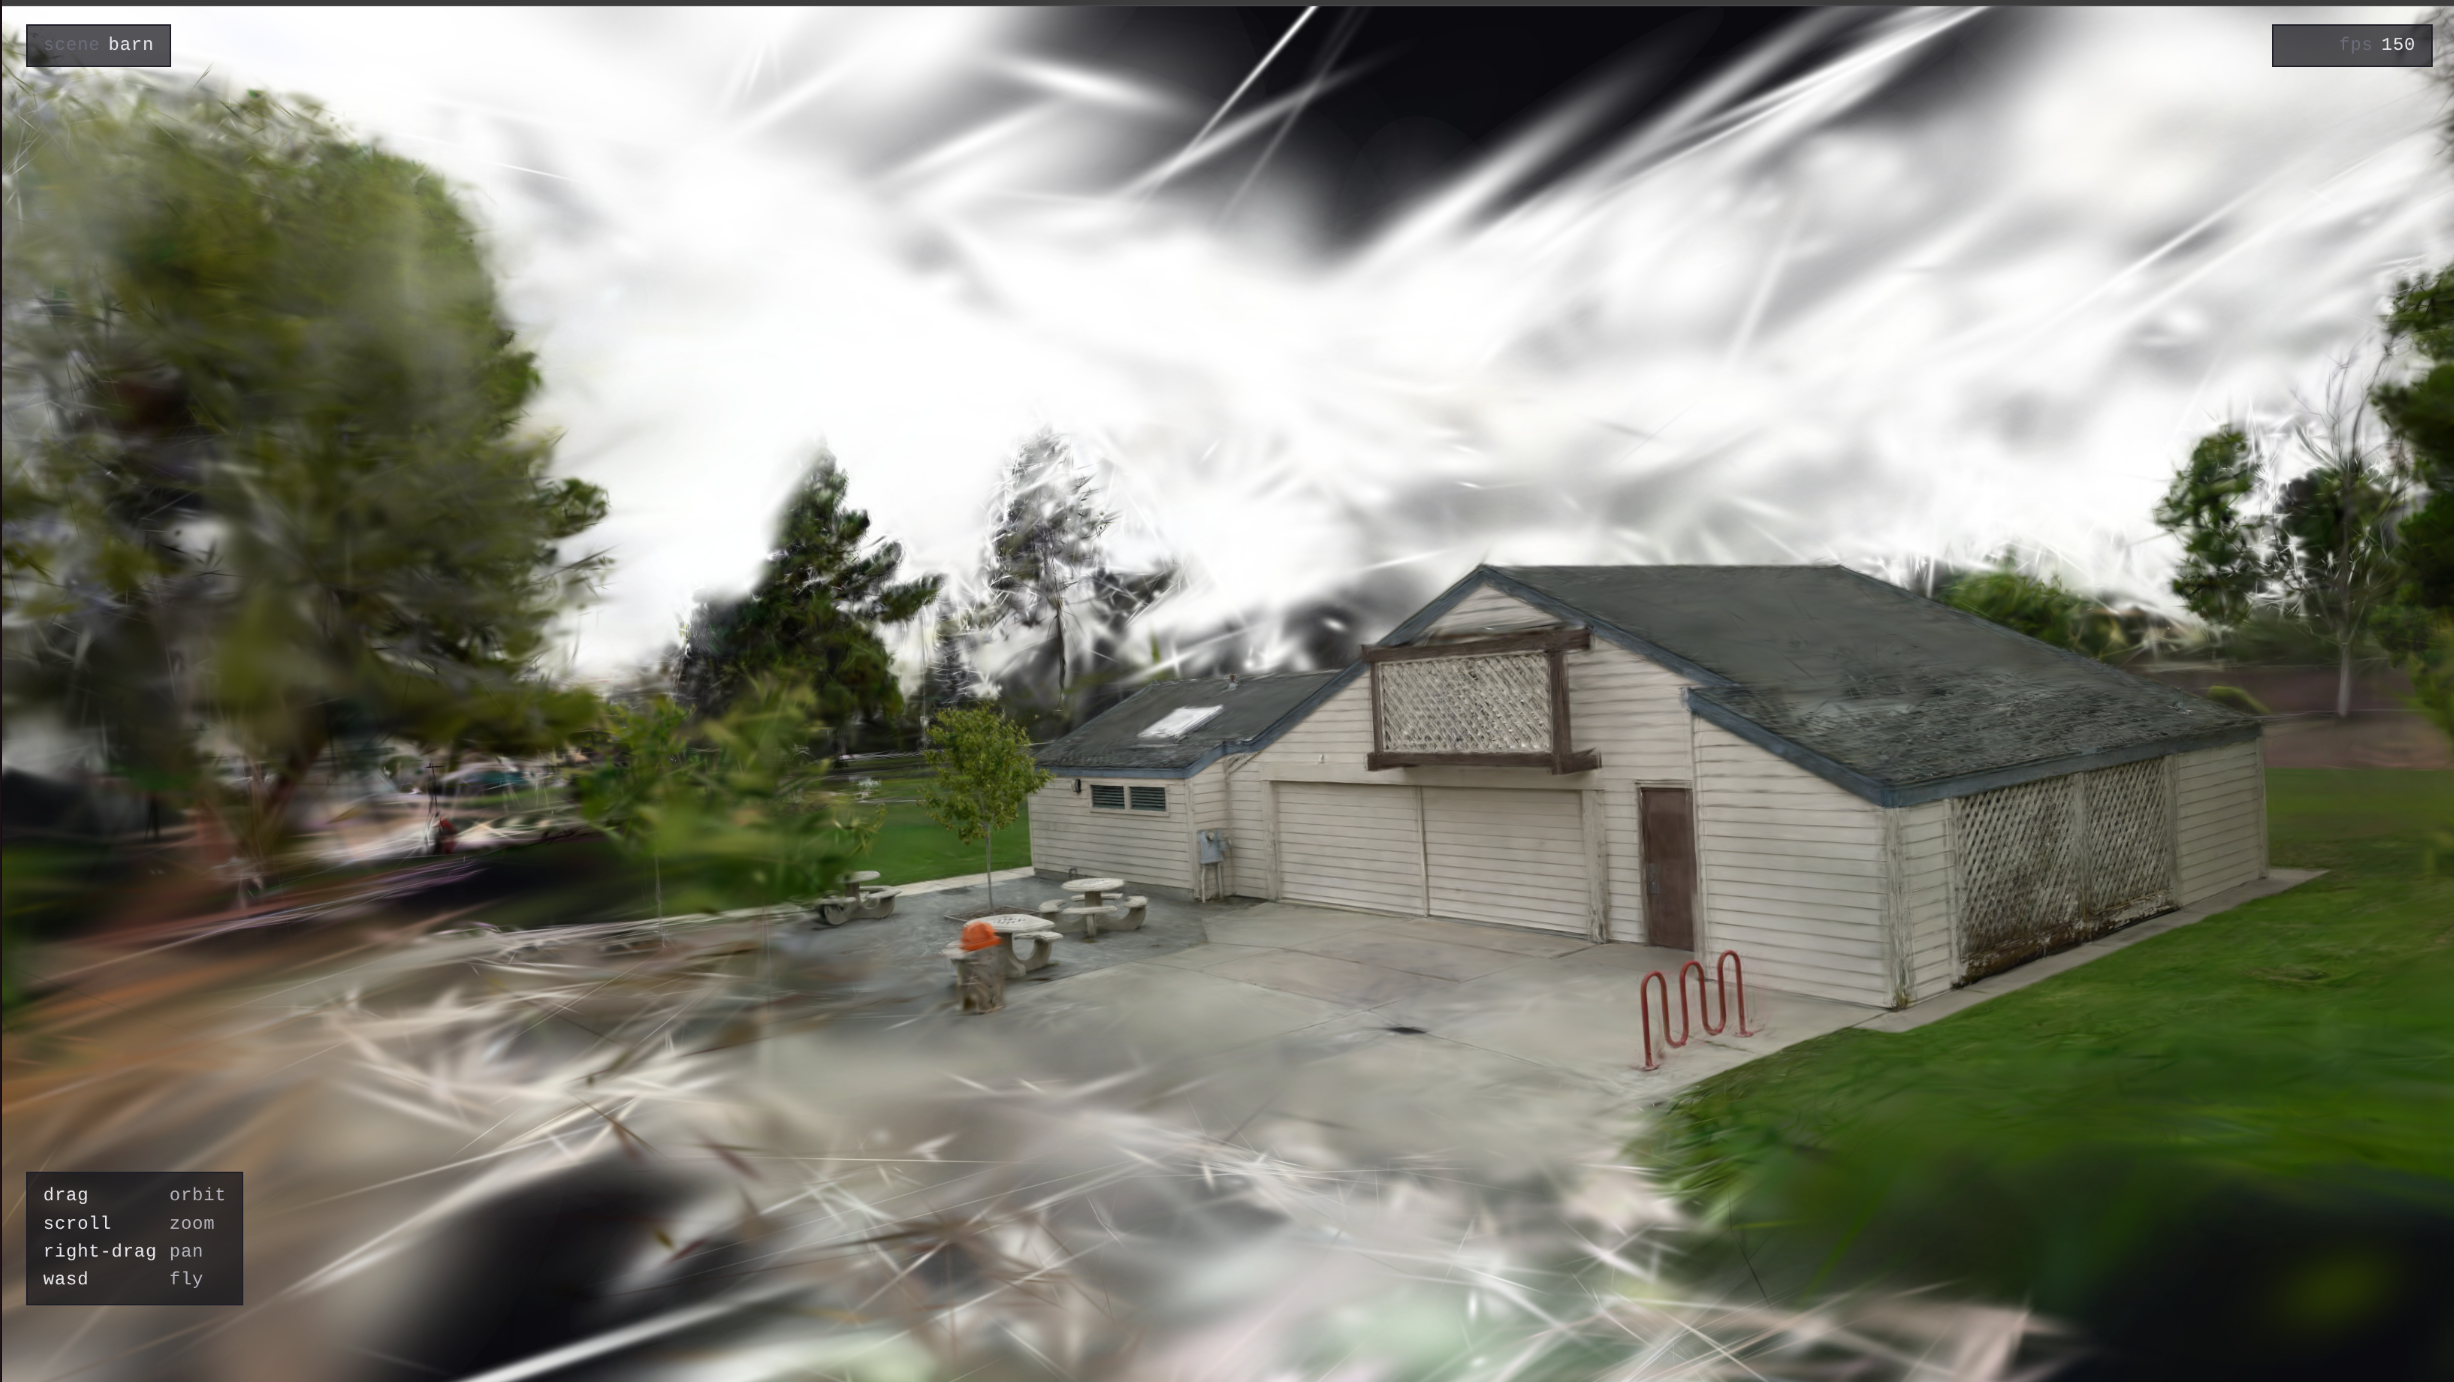
\includegraphics[width=\columnwidth]{viewer_screenshot.png}}
  \caption{The trained barn scene loaded in the browser viewer, showing the HUD with scene name, FPS counter, and built-in controls.}
  \label{fig:viewer}
\end{figure}

\subsection{Debugging the blank-canvas bug}

A non-trivial fraction of the project was spent debugging a failure where the viewer loaded the ksplat successfully, reported 160+ FPS, and still rendered a completely black canvas. We traced it by attaching a Playwright-driven headless Chromium that could inspect WebGL and worker state across page reloads. The root cause turned out to be a single flag: \texttt{gpuAcceleratedSort: true} (the library default) skips uploading Gaussian centers to the CPU sort worker, because it expects the GPU sort path to consume them directly. When the GPU path is not available, the worker's \texttt{uploadedSplatCount} remains zero, the renderer's \texttt{drawRange.count} is also zero, and the canvas is correctly cleared to the background color every frame. Setting \texttt{gpuAcceleratedSort: false} and forcing a \texttt{updateMatrixWorld} call before the first render fixed it. We call this out here because it is the kind of bug that the end-to-end metric (FPS) hides completely.

\section{Discussion and Summary}\label{sec:discussion}

\subsection{What worked}

The combination of a temporally ordered video, sequential COLMAP matching, and 3DGS densification is very effective on a scene with plenty of texture and good camera coverage. 28\,dB PSNR on the first serious training run, from a handheld capture with no special lighting, is better than we expected to get on 8\,GB of VRAM. The 15\,MB ksplat size makes this a reasonable thing to host and send to a browser, not just a local demo.

\subsection{What hurt}

Three specific failure modes dominate the residual error, and they are the same whether the scene is indoors or outdoors. First, \textbf{textureless surfaces} such as painted walls, painted siding, and blank-sky regions give the SIFT matcher nothing to lock onto and the Gaussian density in those regions stays thin; orbiting past them tends to reveal stretched splats. Second, \textbf{specular and view-dependent materials} such as windows, metal fittings, glossy floors, and wet exterior surfaces confuse both SfM and the appearance model at the same time, producing floaters and shimmer. Third, \textbf{sparse coverage of the scene's far side}, that is, the angles the operator never walked around to, produces exactly the stretched low-density Gaussians that hold up when viewed head-on and fall apart the moment the viewer orbits around. None of these are novel to 3DGS; they are the same classes of failure that NeRF and MVS pipelines struggle with, but 3DGS makes them very visible because the representation is explicit.

\subsection{VRAM as the bottleneck}

On our laptop, 8\,GB of VRAM is the binding constraint, not compute. We were forced to train at \texttt{--resolution 2} (640\,px long edge) because full-resolution training OOMs during densification, when the Gaussian count spikes before the prune pass catches up. Training at 12 or 16\,GB would let us take the full-resolution frames and would very likely close some of the gap between our numbers and the original paper's. This is the single largest lever for future work on this hardware class.

\subsection{Future work}

We plan to evaluate the same pipeline on indoor scenes in future work, where window specularity and textureless walls are more severe and sparse corner coverage matters more than it does outside. Beyond that, a few practical improvements are worth pursuing. The ksplat could be streamed progressively instead of fetched as one blob, which \texttt{gaussian-splats-3d} already supports but we disabled for determinism. For larger unbounded outdoor captures, scene-contraction variants \cite{barron2022mipnerf360} would help the current model, which today has to choose between focusing Gaussians on the foreground or the sky. And a CI smoke test that trains 500 iterations on a five-frame subset and checks that the numbers come back in a sane range would catch toolchain drift the moment it happens, instead of after a full 30k-iteration run.

\subsection{Summary}

We built a complete, reproducible, open-source pipeline from raw webcam video to a browser-deliverable 3D Gaussian Splatting scene, running end-to-end on a single laptop GPU. On the barn scene we reach 28.11\,dB PSNR, 0.879 SSIM, and 0.120 LPIPS on held-out views in 17 minutes of training, and deliver a 15\,MB ksplat that renders at real-time rates in the browser. The remaining quality gap is dominated by a small number of well-understood failure modes and by a hard 8\,GB VRAM ceiling on training resolution. All code, scripts, and environment files, plus a one-command reproduction of the barn result, are available at \url{https://github.com/Meetjain-0201/3dgs-outdoor-reconstruction}.

\newpage

\begin{thebibliography}{00}
\bibitem{mildenhall2020nerf} B. Mildenhall, P. P. Srinivasan, M. Tancik, J. T. Barron, R. Ramamoorthi, and R. Ng, ``NeRF: Representing scenes as neural radiance fields for view synthesis,'' in \textit{Proc. European Conf. Comput. Vis. (ECCV)}, 2020, pp. 405--421.

\bibitem{kerbl20233dgs} B. Kerbl, G. Kopanas, T. Leimk{\"u}hler, and G. Drettakis, ``3D Gaussian splatting for real-time radiance field rendering,'' \textit{ACM Trans. Graph.}, vol. 42, no. 4, pp. 1--14, Jul. 2023.

\bibitem{schonberger2016sfm} J. L. Sch{\"o}nberger and J.-M. Frahm, ``Structure-from-motion revisited,'' in \textit{Proc. IEEE Conf. Comput. Vis. Pattern Recognit. (CVPR)}, 2016, pp. 4104--4113.

\bibitem{lowe2004sift} D. G. Lowe, ``Distinctive image features from scale-invariant keypoints,'' \textit{Int. J. Comput. Vis.}, vol. 60, no. 2, pp. 91--110, Nov. 2004.

\bibitem{schonberger2016mvs} J. L. Sch{\"o}nberger, E. Zheng, M. Pollefeys, and J.-M. Frahm, ``Pixelwise view selection for unstructured multi-view stereo,'' in \textit{Proc. European Conf. Comput. Vis. (ECCV)}, 2016, pp. 501--518.

\bibitem{mueller2022instantngp} T. M{\"u}ller, A. Evans, C. Schied, and A. Keller, ``Instant neural graphics primitives with a multiresolution hash encoding,'' \textit{ACM Trans. Graph.}, vol. 41, no. 4, pp. 1--15, Jul. 2022.

\bibitem{barron2022mipnerf360} J. T. Barron, B. Mildenhall, D. Verbin, P. P. Srinivasan, and P. Hedman, ``Mip-NeRF 360: Unbounded anti-aliased neural radiance fields,'' in \textit{Proc. IEEE Conf. Comput. Vis. Pattern Recognit. (CVPR)}, 2022, pp. 5470--5479.

\bibitem{wang2004ssim} Z. Wang, A. C. Bovik, H. R. Sheikh, and E. P. Simoncelli, ``Image quality assessment: From error visibility to structural similarity,'' \textit{IEEE Trans. Image Process.}, vol. 13, no. 4, pp. 600--612, Apr. 2004.

\bibitem{zhang2018lpips} R. Zhang, P. Isola, A. A. Efros, E. Shechtman, and O. Wang, ``The unreasonable effectiveness of deep features as a perceptual metric,'' in \textit{Proc. IEEE Conf. Comput. Vis. Pattern Recognit. (CVPR)}, 2018, pp. 586--595.

\bibitem{kellogg2023viewer} M. Kellogg, ``gaussian-splats-3d: Three.js-based implementation of a 3D Gaussian splatting viewer,'' GitHub repository, 2023. [Online]. Available: \url{https://github.com/mkkellogg/GaussianSplats3D}
\end{thebibliography}

\end{document}
